\section{10. Tabellen und Graphen \texorpdfstring{$\star$}{*}}

\begin{minipage}{\linewidth}
\Tab Spezielle Werte der Trigonometrischen Funktionen

\begin{tabular}{l | c c c c c c}
    $\theta$ (rad) & $0$ & $\frac{\pi}{6}$ & $\frac{\pi}{4}$ & $\frac{\pi}{3}$ & $\frac{\pi}{2}$ & $\pi$ \\[1ex]
    $\theta$ ($^\circ$) & $0^\circ$ & $30^\circ$ & $45^\circ$ & $60^\circ$ & $90^\circ$ & $180^\circ$ \\[0.5ex]
    \hline
    $\sin\theta$ & $0$ & $\frac{1}{2}$ & $\frac{\sqrt{2}}{2}$ & $\frac{\sqrt{3}}{2}$ & $1$ & $0$ \\[1ex]
    $\cos\theta$ & $1$ & $\frac{\sqrt{3}}{2}$ & $\frac{\sqrt{2}}{2}$ & $\frac{1}{2}$ & $0$ & $-1$ \\[1ex]
    $\tan\theta$ & $0$ & $\frac{\sqrt{3}}{3}$ & $1$ & $\sqrt{3}$ & N/A & $0$
\end{tabular}
\end{minipage}

\begin{minipage}{\linewidth}
\Tab Trigonometrische Identitäten
\begin{itemize}
    \item \key{Definitionen}: $\tan x = \frac{\sin x}{\cos x}$, $\;\cot x = \frac{\cos x}{\sin x} = \frac{1}{\tan x}$
    \item $\sec x = \frac{1}{\cos x}$, $\;\csc x = \frac{1}{\sin x}$
    \item \key{Pythagoras}: $\sin^2x + \cos^2x = 1$
    \item $1+\tan^2x=\sec^2x$, $\;1+\cot^2x=\csc^2x$
    \item \key{Parität}: $\sin(-x)=-\sin x$, $\;\cos(-x)=\cos x$
    \item \key{Summe}: $\sin(a\pm b)=\sin a\cos b\pm\cos a\sin b$
    \item $\cos(a\pm b)=\cos a\cos b\mp\sin a\sin b$
    \item \key{Doppelwinkel}: $\sin(2x)=2\sin x\cos x$
    \item $\cos(2x)=\cos^2x-\sin^2x=2\cos^2x-1=1-2\sin^2x$
    \item \key{Halbwinkel}: $\sin^2\frac{x}{2}=\frac{1-\cos x}{2}$, $\;\cos^2\frac{x}{2}=\frac{1+\cos x}{2}$
    \item $\tan\frac{x}{2}=\frac{1-\cos x}{\sin x}=\frac{\sin x}{1+\cos x}$
    \item \key{Komplexe Form (Euler)}: $\cos x=\frac{e^{ix}+e^{-ix}}{2}$, $\;\sin x=\frac{e^{ix}-e^{-ix}}{2i}$
\end{itemize}
\end{minipage}

\begin{minipage}{\linewidth}
\Bild Graphen von Trigonometrischen Funktionen

\begin{center}
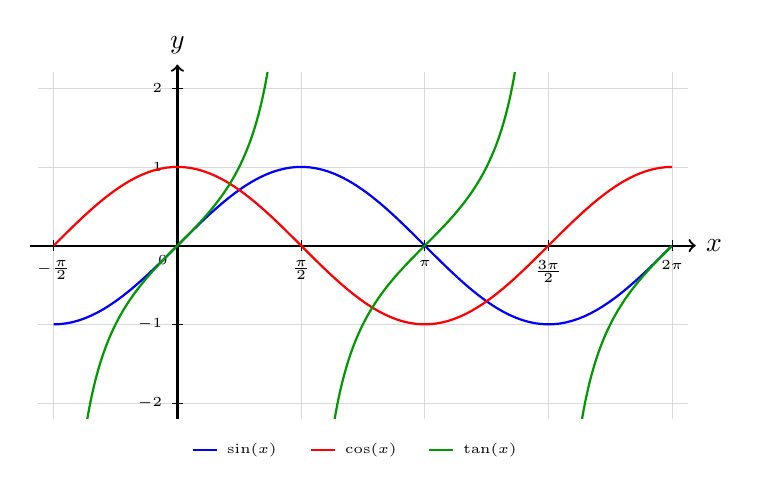
\begin{tikzpicture}
    \draw[very thin, gray!30, xstep={pi/2}, ystep=1] ({-pi/2 - 0.2}, -2.2) grid ({2*pi + 0.2}, 2.2);

    \draw[->, thick] ({-pi/2 - 0.3}, 0) -- ({2*pi + 0.3}, 0) node[right] {$x$};
    \draw[->, thick] (0, -2.2) -- (0, 2.3) node[above] {$y$};

    \draw ({-pi/2}, 2pt) -- ({-pi/2}, -2pt) node[below, font=\tiny] {$-\frac{\pi}{2}$};
    \draw ({pi/2}, 2pt)  -- ({pi/2}, -2pt)  node[below, font=\tiny] {$\frac{\pi}{2}$};
    \draw ({pi}, 2pt)    -- ({pi}, -2pt)    node[below, font=\tiny] {$\pi$};
    \draw ({3*pi/2}, 2pt)-- ({3*pi/2}, -2pt)node[below, font=\tiny] {$\frac{3\pi}{2}$};
    \draw ({2*pi}, 2pt)  -- ({2*pi}, -2pt)  node[below, font=\tiny] {$2\pi$};

    \foreach \y in {-2, -1, 1, 2}
        \draw (2pt, \y) -- (-2pt, \y) node[left, font=\tiny] {$\y$};
    \node[below left, font=\tiny] at (0,0) {$0$};

    \begin{scope}
        \clip ({-pi/2 - 0.2}, -2.2) rectangle ({2*pi + 0.1}, 2.2);

        \draw[thick, blue, domain={-pi/2}:{2*pi}, samples=100] 
            plot (\x, {sin(\x r)});

        \draw[thick, red, domain={-pi/2}:{2*pi}, samples=100] 
            plot (\x, {cos(\x r)});

        \draw[thick, green!60!black, domain=-1.4:1.4, samples=100] 
            plot (\x, {tan(\x r)});
        \draw[thick, green!60!black, domain=1.75:4.55, samples=100] 
            plot (\x, {tan(\x r)});
        \draw[thick, green!60!black, domain=4.9:6.28, samples=50] 
            plot (\x, {tan(\x r)});
    \end{scope}

    \begin{scope}[shift={(0.2, -2.6)}, font=\tiny]
        \draw[thick, blue] (0,0) -- (0.3,0) node[right, black] {$\sin(x)$};
        \draw[thick, red] (1.5,0) -- (1.8,0) node[right, black] {$\cos(x)$};
        \draw[thick, green!60!black] (3.0,0) -- (3.3,0) node[right, black] {$\tan(x)$};
    \end{scope}
\end{tikzpicture}
\end{center}
\end{minipage}

\begin{minipage}{\linewidth}
\Bild Graphen von Trigonometrischen Inversen

\begin{center}
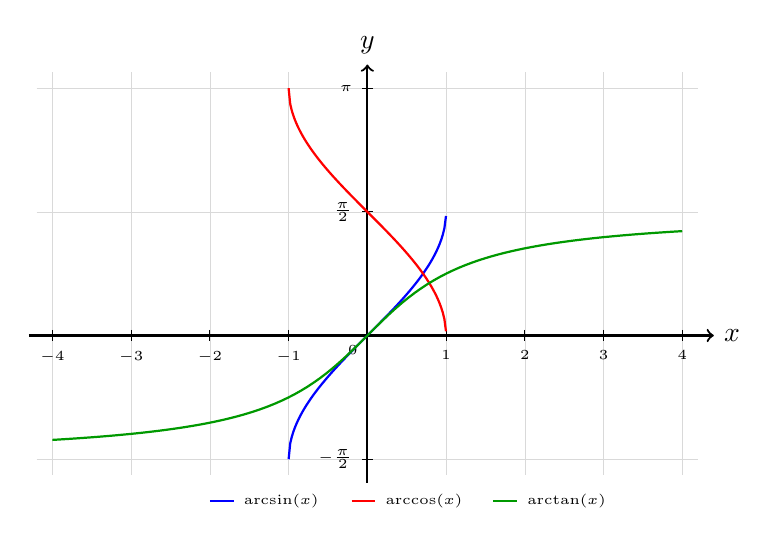
\begin{tikzpicture}
    \draw[very thin, gray!30, xstep=1, ystep={pi/2}] (-4.2, {-pi/2 - 0.2}) grid (4.2, {pi + 0.2});

    \draw[->, thick] (-4.3, 0) -- (4.4, 0) node[right] {$x$};
    \draw[->, thick] (0, {-pi/2 - 0.3}) -- (0, {pi + 0.3}) node[above] {$y$};

    \foreach \x in {-4, -3, -2, -1, 1, 2, 3, 4}
        \draw (\x, 2pt) -- (\x, -2pt) node[below, font=\tiny] {$\x$};

    \draw (2pt, {-pi/2}) -- (-2pt, {-pi/2}) node[left, font=\tiny] {$-\frac{\pi}{2}$};
    \draw (2pt, {pi/2})  -- (-2pt, {pi/2})  node[left, font=\tiny] {$\frac{\pi}{2}$};
    \draw (2pt, {pi})    -- (-2pt, {pi})    node[left, font=\tiny] {$\pi$};
    \node[below left, font=\tiny] at (0,0) {$0$};

    \begin{scope}
        \clip (-4.2, {-pi/2 - 0.2}) rectangle (4.2, {pi + 0.2});

        \draw[thick, blue, domain=-1:1, samples=100] 
            plot (\x, {rad(asin(\x))});

        \draw[thick, red, domain=-1:1, samples=100] 
            plot (\x, {rad(acos(\x))});

        \draw[thick, green!60!black, domain=-4:4, samples=100] 
            plot (\x, {rad(atan(\x))});
    \end{scope}

    \begin{scope}[shift={(-2.0, -2.1)}, font=\tiny]
        \draw[thick, blue] (0,0) -- (0.3,0) node[right, black] {$\arcsin(x)$};
        \draw[thick, red] (1.8,0) -- (2.1,0) node[right, black] {$\arccos(x)$};
        \draw[thick, green!60!black] (3.6,0) -- (3.9,0) node[right, black] {$\arctan(x)$};
    \end{scope}
\end{tikzpicture}
\end{center}
\end{minipage}

\begin{minipage}{\linewidth}
\Bild Graphen von Exponentialfunktionen (und $\frac{1}{x}$ just because)

\begin{center}
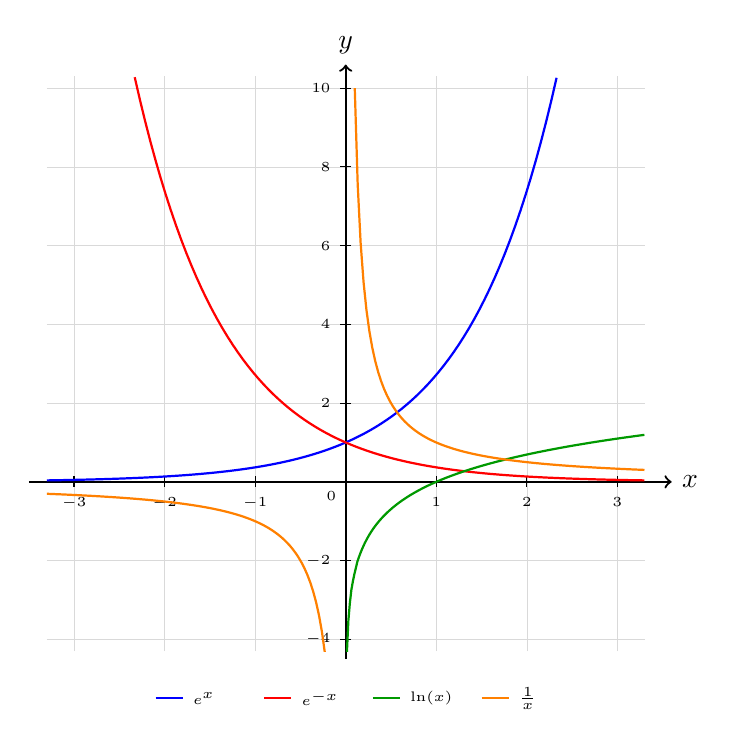
\begin{tikzpicture}[x=1.15cm, y=0.5cm]
    % Grid matching xstep = 1 and ystep = 2
    \draw[very thin, gray!30, xstep=1, ystep=2] (-3.3, -4.3) grid (3.3, 10.3);

    % Axes
    \draw[->, thick] (-3.5, 0) -- (3.6, 0) node[right] {$x$};
    \draw[->, thick] (0, -4.5) -- (0, 10.6) node[above] {$y$};

    % X-Axis Ticks (Steps of 1 from -3 to 3)
    \foreach \x in {-3, -2, -1, 1, 2, 3}
        \draw (\x, 2pt) -- (\x, -2pt) node[below, font=\tiny] {$\x$};

    % Y-Axis Ticks (Steps of 2 from -4 to 10)
    \foreach \y in {-4, -2, 2, 4, 6, 8, 10}
        \draw (2pt, \y) -- (-2pt, \y) node[left, font=\tiny] {$\y$};
    \node[below left, font=\tiny] at (0,0) {$0$};

    % Clip plot region
    \begin{scope}
        \clip (-3.3, -4.3) rectangle (3.3, 10.3);

        % 1. e^x (Blue)
        \draw[thick, blue, domain=-3.3:2.33, samples=100] 
            plot (\x, {exp(\x)});

        % 2. e^-x (Red)
        \draw[thick, red, domain=-2.33:3.3, samples=100] 
            plot (\x, {exp(-\x)});

        % 3. ln(x) (Green)
        \draw[thick, green!60!black, domain=0.013:3.3, samples=200] 
            plot (\x, {ln(\x)});

        % 4. 1/x (Orange) - Split domain to avoid x = 0 asymptote
        \draw[thick, orange, domain=-3.3:-0.1, samples=100] 
            plot (\x, {1/\x});
        \draw[thick, orange, domain=0.1:3.3, samples=100] 
            plot (\x, {1/\x});
    \end{scope}

    % Legend
    \begin{scope}[shift={(0.0, -5.5)}, font=\tiny]
        \draw[thick, blue] (-2.1,0) -- (-1.8,0) node[right, black] {$e^x$};
        \draw[thick, red] (-0.9,0) -- (-0.6,0) node[right, black] {$e^{-x}$};
        \draw[thick, green!60!black] (0.3,0) -- (0.6,0) node[right, black] {$\ln(x)$};
        \draw[thick, orange] (1.5,0) -- (1.8,0) node[right, black] {$\frac{1}{x}$};
    \end{scope}

\end{tikzpicture}
\end{center}
\end{minipage}

\begin{minipage}{\linewidth}
\Tab Wichtige Grenzwerte

\begin{tabular}{l c r}
    $\lim f(x)$ & Grenzwert $L$ & Bedingung \\
    \hline
    $\lim\limits_{n\to\infty} \frac{\ln n}{n}$ & $0$ & \\[1ex]
    $\lim\limits_{n\to\infty} \sqrt[n]{n}$ & $1$ & \\[1ex]
    $\lim\limits_{n\to\infty} \sqrt[n]{x}$ & $1$ & $x > 0$ \\[1ex]
    $\lim\limits_{n\to\infty} \left(1 + \frac{x}{n}\right)^n$ & $e^x$ & $x \in \mathbb{R}$ \\[1ex]
    $\lim\limits_{n\to\infty} \frac{x^n}{n!}$ & $0$ & $x \in \mathbb{R}$ \\[0.5ex]
    \hline
    $\lim\limits_{n\to\infty} x^n$ & $0$ & $|x| < 1$ \\[1ex]
    $\lim\limits_{n\to\infty} \frac{n^k}{a^n}$ & $0$ & $a > 1, k \in \mathbb{R}$ \\[1ex]
    $\lim\limits_{n\to\infty} \frac{a^n}{n!}$ & $0$ & $a > 0$ \\[1ex]
    $\lim\limits_{n\to\infty} \frac{n!}{n^n}$ & $0$ & \\[1ex]
    $\lim\limits_{n\to\infty} \sqrt[n]{a^n + b^n}$ & $\max(a, b)$ & $a, b \ge 0$ \\
    \hline
    $\lim\limits_{x\to 0} \frac{\sin x}{x}$ & $1$ & $x \neq 0$ \\[1ex]
    $\lim\limits_{x\to 0} \frac{1 - \cos x}{x^2}$ & $\frac{1}{2}$ & $x \neq 0$ \\[1ex]
    $\lim\limits_{x\to 0} \frac{e^x - 1}{x} = \lim\limits_{x\to 0} \frac{e^x}{x + 1}$ & $1$ & $x \neq 0$ \\[1ex]
    $\lim\limits_{x\to 0} \frac{\ln(1 + x)}{x}$ & $1$ & $x > -1, x \neq 0$ \\[1ex]
    $\lim\limits_{x\to 0} \frac{(1 + x)^k - 1}{x}$ & $k$ & $k \in \mathbb{R}, x \neq 0$ \\[0.5ex]
    \hline
    $\lim\limits_{x\to 0^+} x^x$ & $1$ & \\[1ex]
    $\lim\limits_{x\to 0^+} x^a \ln x$ & $0$ & $a > 0$ \\[1ex]
    $\lim\limits_{x\to\infty} \frac{(\ln x)^k}{x^a}$ & $0$ & $a > 0, k \in \mathbb{R}$
\end{tabular}
\end{minipage}

\begin{minipage}{\linewidth}
\Tab Wichtige Maclaurin-Reihen

\begin{tabular}{l c c r}
    $f(x)$ & Entwicklung & Summenform & Bedingung \\
    \hline
    $e^x$ & $1 + x + \frac{x^2}{2!} + \dots$ & $\sum_{k=0}^\infty \frac{x^k}{k!}$ & $x \in \mathbb{R}$ \\[1ex]
    $\cos x$ & $1 - \frac{x^2}{2!} + \frac{x^4}{4!} - \dots$ & $\sum_{k=0}^\infty (-1)^k \frac{x^{2k}}{(2k)!}$ & $x \in \mathbb{R}$ \\[1ex]
    $\sin x$ & $x - \frac{x^3}{3!} + \frac{x^5}{5!} - \dots$ & $\sum_{k=0}^\infty (-1)^k \frac{x^{2k+1}}{(2k+1)!}$ & $x \in \mathbb{R}$ \\[1ex]
    $\cosh x$ & $1 + \frac{x^2}{2!} + \frac{x^4}{4!} + \dots$ & $\sum_{k=0}^\infty \frac{x^{2k}}{(2k)!}$ & $x \in \mathbb{R}$ \\[1ex]
    $\sinh x$ & $x + \frac{x^3}{3!} + \frac{x^5}{5!} + \dots$ & $\sum_{k=0}^\infty \frac{x^{2k+1}}{(2k+1)!}$ & $x \in \mathbb{R}$ \\[1ex]
    \hline
    $\frac{1}{1-x}$ & $1 + x + x^2 + \dots$ & $\sum_{k=0}^\infty x^k$ & $|x| < 1$ \\[1ex]
    $\frac{1}{1+x}$ & $1 - x + x^2 - \dots$ & $\sum_{k=0}^\infty (-1)^k x^k$ & $|x| < 1$ \\[1ex]
    $\ln(1+x)$ & $x - \frac{x^2}{2} + \frac{x^3}{3} + \dots$ & $\sum_{k=1}^\infty (-1)^{k-1} \frac{x^k}{k}$ & $-1 < x \le 1$ \\[1ex]
    $\arctan x$ & $x - \frac{x^3}{3} + \frac{x^5}{5} - \dots$ & $\sum_{k=0}^\infty (-1)^k \frac{x^{2k+1}}{2k+1}$ & $|x| \le 1$ \\[1ex]
    $(1+x)^\alpha$ & $1 + \alpha x + \dots$ & $\sum_{k=0}^\infty \binom{\alpha}{k} x^k$ & $|x| < 1$ \\
\end{tabular}
\end{minipage}

\begin{minipage}{\linewidth}
\Tab Ableitungen und Stammfunktionen

\begin{tabular}{l c r}
    $f(x)$ & $f'(x)$ & $\int f(x) \, dx (+ C)$ \\
    \hline
    $x^n \ (n \neq -1)$ & $n x^{n-1}$ & $\frac{x^{n+1}}{n+1}$ \\[1ex]
    $\sqrt{x}$ & $\frac{1}{2\sqrt{x}}$ & $\frac{2}{3}x\sqrt{x}$ \\[1ex]
    $\sqrt[n]{x}$ & $\frac{1}{n\sqrt[n]{x^{n-1}}}$ & $\frac{n}{n+1}x\sqrt[n]{x}$ \\[1ex]
    $\frac{1}{x}$ & $-\frac{1}{x^2}$ & $\ln|x|$ \\[1ex]
    $e^x$ & $e^x$ & $e^x$ \\[1ex]
    $a^x$ & $a^x \ln a$ & $\frac{a^x}{\ln a}$ \\[1ex]
    $\ln x$ & $\frac{1}{x}$ & $x \ln x - x$ \\[0.5ex]
    \hline
    $\sin x$ & $\cos x$ & $-\cos x$ \\[1ex]
    $\cos x$ & $-\sin x$ & $\sin x$ \\[1ex]
    $\tan x$ & $\sec^2 x$ & $-\ln|\cos x|$ \\[1ex]
    $\sec x$ & $\sec x \tan x$ & $\ln|\sec x + \tan x|$ \\[1ex]
    $\csc x$ & $-\csc x \cot x$ & $-\ln|\csc x + \cot x|$ \\[1ex]
    $\cot x$ & $-\csc^2 x$ & $\ln|\sin x|$ \\
    \hline
    $\arcsin x$ & $\frac{1}{\sqrt{1-x^2}}$ & $x \arcsin x + \sqrt{1-x^2}$ \\[1ex]
    $\arccos x$ & $-\frac{1}{\sqrt{1-x^2}}$ & $x \arccos x - \sqrt{1-x^2}$ \\[1ex]
    $\arctan x$ & $\frac{1}{1+x^2}$ & $x \arctan x - \frac{1}{2}\ln(1+x^2)$ \\[0.5ex]
    \hline
    $\sinh x$ & $\cosh x$ & $\cosh x$ \\[1ex]
    $\cosh x$ & $\sinh x$ & $\sinh x$ \\[1ex]
    $\tanh x$ & $\operatorname{sech}^2 x$ & $\ln(\cosh x)$ \\
\end{tabular}
\end{minipage}
